\chapter{Propiedades de la Membrana de  \textit{Staphyloccocus aureus} y Resistencia de la Bacteria}
\section{La membrana Bacteriana y sus compuestos presentes}\label{ss:mem}
Seg\'{u}n el tipo de membrana que posean las bacterias, est\'{a}s pueden clasificarse en dos grandes clases: las bacterias Gram positivas y las bacterias Gram negativas. Las bacterias Gram positivas poseen una sola bicapa lip\'{i}dica envuelta en una capa compuesta por unos pol\'{i}meros de az\'{u}cares y amino\'{a}cidos llamados peptidoglicando (ver figura \ref{fig:mem}), mientras que las membranas de bacterias Gram negativa poseen dos bicapas lip\'{i}dicas. Ya que \textit{Staphylococcus aureus} es una bacteria Gram positiva se discutir\'{a} principalmente la composici\'{o}n de la membrana de las bacterias Gram Positivas.\\

\begin{figure}[h]
\begin{center}
  \includegraphics[scale=0.3]{Kap2/grampos1.png}
    \includegraphics[scale=0.15]{Kap2/grampos2.png}
  \caption{Imagen  de la membrana de una bacteria Gram positiva. Tomado de \cite{Nelson2011}.}
  \label{fig:mem}
\end{center}
\end{figure}
La bicapa lip\'{i}dica es una membrana presente en todos las c\'{e}lulas, la cual est\'{a} compuesta mayoritariamente por l\'{i}pidos. Los l\'{i}pidos se acomodan de tal manera que el espesor de la membrana sea de dos l\'{i}pidos de grosor.  En su mayor\'{i}a, con excepciones como los esteroles, los l\'{i}pidos est\'{a}n compuestos por una o varias cadenas de \'{a}cidos grasos no polares (cadenas hidrocarbonadas con carboxilo) unidas a diferentes sustituyentes polares los cuales pueden presentar carga o no a pH fisiol\'{o}gico. De acuerdo a los sustituyentes y al tipo de \'{a}cidos grasos, cada l\'{i}pido presenta propiedades fisicoqu\'{i}micas espec\'{i}ficas como la carga total, la polaridad, y el largo que lo distinguen a nivel biof\'{i}sico con los otros l\'{i}pidos.\\

Los \'{a}cidos grasos normalmente no se encuentran libres sino que est\'{a}n unidos por parejas o en d\'{i}meros. Uno de los agentes que une los \'{a}cidos grasos es el glicerol, en donde cada \'{a}cido graso se une mediante enlaces covalentes al grupo glicerol \cite{Bagatolli2017VidaGrasas}. Como el glicerol tiene 3 hidroxilos, habr\'{a} un m\'{a}ximo de tres \'{a}cidos grasos que esterificar\'{a}n al glicerol. En el caso de los triacilgliceroles (triglic\'{e}ridos) los tres \'{a}cidos grasos est\'{a}n unidos al glicerol. En otros casos, hay solamente dos \'{a}cidos grasos unidos a un glicerol y uno de los hidroxilos que quedan libres es sustituido con un grupo fosfato. Los l\'{i}pidos que tengan varios \'{a}cidos grasos unidos por gliceroles y que tengan fosfatos se denominan \textit{glicerofosfol\'{i}pidos}.\\

%A parte de los l\'{i}pidos, las bicapas lip\'{i}dicas de las bacterias tambi\'{e}n poseen prote\'{i}nas de membrana y otras mol\'{e}culas como glicol\'{i}pidos y carotenos. Tambi\'{e}n pueden poseer
Adicionalmente, los posibles sustituyentes se unen al grupo fosfato d\'{a}ndole al glicerofosfol\'{i}pido sus propiedades caracter\'{i}sticas. Algunos de estos son el hidr\'{o}geno, la colina, la serina, la etalonamina e incluso el glicerol. La f\'{o}rmula de los sustituyentes nombrados ac\'{a} puede verse en la tabla \ref{tab:polar}. A pH fisiol\'{o}gico la colina y la etalonamina tienen carga positiva, mientras que la serina tiene carga negativa. El glicerol a pH fisiol\'{o}gico est\'{a} descargado.\\

\begin{table}[]
    \centering
    \begin{tabular}{c}
  \includegraphics[scale=0.4]{Kap2/headgroups.png}
    \end{tabular}
    \caption{Algunos sustituyentes para el grupo polar de los glicerofosfol\'{i}pidos. Figura tomada de \cite{Bagatolli2017VidaGrasas}.}
    \label{tab:polar}
\end{table}

Los l\'{i}pidos forman bicapas debido a la presencia del agua ya que al ser mol\'{e}culas anfip\'{a}ticas (combinando motivos polares y apolares) se orientan con respecto a esta. La parte hidrof\'{i}lica del l\'{i}pido interact\'{u}a con el agua mientras que la parte hidrof\'{o}bica no interact\'{u}a con esta, lo que induce reorientaci\'{o}n y agregaci\'{o}n de los l\'{i}pidos. Estas interacciones hacen que sea m\'{a}s estable encontrar los l\'{i}pidos inmersos en el agua formando agregados sin mezclarse con el agua. La interacci\'on lateral entre estas mol\'eculas se da a trav\'es de fuerzas no covalentes lo que le confiere propiedades de cristal l\'iquido caracterizado por la capacidad de presentar transiciones de fase t\'{e}rmicas de s\'olido a l\'iquido y difusi\'{o}n lateral. \\
\section{Composici\'{o}n de la bicapa lip\'{i}dica de \textit{Staphylococcus aureus}}
En el caso de las bacterias Gram positivas, en particular de las pertenecientes al grupo taxon\'{o}mico de las firmicutes, se ha encontrado que en la mayor\'{i}a de sus especies, las membranas bacterianas contienen principalmente fosfatidilgliceroles (PG),cardiolipina (CL) y en algunas pueden contener o no fosfatidiletalnamina (PE). Ya que \textit{Staphylococcus aureus} pertenece a este grupo taxon\'{o}mico, la bacteria est\'{a} compuesta principalmente por fosfatidilgliceroles (PG), cardiolipina (CL) y adicionalmente tiene otros l\'{i}pidos como los lifosfoglicandos (LPG) y los glicopeptidol\'{i}pidos (GPL) \cite{Sohlenkamp2015BacterialPathways}. \\

En la figura \ref{fig:lipids} se muestra la f\'{o}rmula estructural dos fosfatidilgliceroles presentes en \textit{Staphylococcus aureus} as\'{i} como la cardiolipina, que es un d\'{i}mero de fosfatidilgliceroles.  Dimiristoilfosphatidilglicerol (DMPG) es un l\'{i}pido que tiene un glicerol unido a dos miristoil (provenientes del \'{a}cido mir\'{i}stico) 14:0 mientras que Dipalmitoilfosphatidilglicerol (DPPG) es un l\'{i}pido con el fosfatidilglicerol unido a dos palmitoil. Tanto DMPG como DPPG poseen en la cabeza polar un grupo fosfato y  un glicerol. Esta caracter\'{i}stica hace que DMPG y DPPG tengan una carga neta negativa a pH fisiol\'{o}gico.\\

\begin{figure}
\begin{center}
    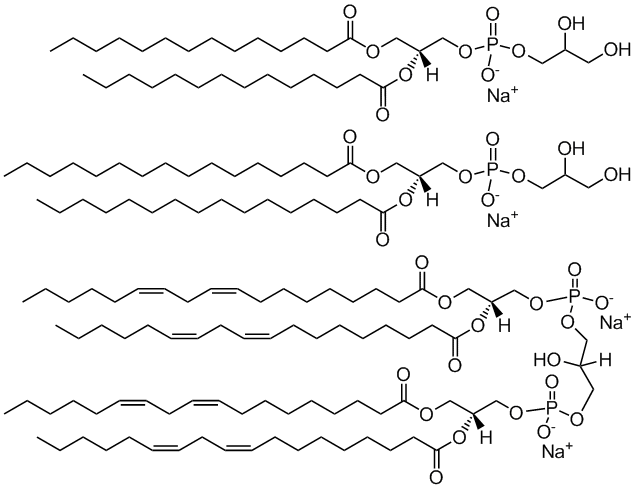
\includegraphics[scale=0.7]{Kap2/lipids.png}
    \put(-130,80){a)}
    \put(-130,50){b)}
    \put(-130,20){c)}
  \caption{ F\'{o}rmulas estructurales de a)  Dimiristoilfosfatidilglicerol (DMPG), b)  Dimiristoilfosfatidilglicerol (DPPG) y c) cardiolipina. Figuras tomadas de \cite{AvantiPolarLipidsInc.2014AvantiLipids}.}
  \label{fig:lipids}
\end{center}
\end{figure}
Las membranas lip\'{i}dicas adem\'{a}s de tener l\'{i}pidos contienen otros tipos de biomol\'{e}culas como los carotenoides, las prote\'{i}nas y los glicol\'{i}pidos que tienen relevancia fisiol\'{o}gica en la c\'{e}lula. Los carotenoides en particular pigmentan las c\'{e}lulas. En el caso de \textit{Staphylococcus aureus} se ha descubierto que los carotenoides juegan un papel importante en la integridad de la membrana celular y protegen a la bacteria frente a estr\'{e}s oxidativo \cite{Nagendra2011}.\\

La protecci\'{o}n de la bacteria est\'{a} basada en cierto tipo de cadena de enlaces dobles conjugados, conocida como cadena poli\'{e}nica, la cual poseen los carotenoides, ver \cite{Nelson2011} y \cite{Gruszecki2004CarotenoidsProperties}. Estos enlaces dobles conjugados permiten la absorci\'{o}n de radicales que se encuentran en el medio y ayudan a la fotoprotecci\'{o}n de la bacteria. La fotoprotecci\'{o}n de la bacteria es interesante desde el punto de vista espectrosc\'{o}pico porque  hace que algunos carotenos absorban en el espectro del infrarrojo y emitan el espectro visible tal como se ve en los espectros mostrados en \cite{Gruszecki2004CarotenoidsProperties} y \cite{Wimpfheimer2015ACompounds}. Como emiten en el espectro visible esto hace que los carotenoides tengan la propiedad de ser pigmentos. Una consecuencia de la presencia de los carotenoides, es la protecci\'{o}n de los carotenoides en la membrana, la cual se ve reflejada por un aumento de su rigidez, \cite{Gruszecki2004CarotenoidsProperties}, de forma similar al papel que juega el colesterol en la membrana eucari\'{o}tica, ver \cite{Bagatolli2017VidaGrasas}.\\

Uno de los carotenoides m\'{a}s relevantes en \textit{Staphylococcus aureus} es la estafiloxantina, la cual le da el nombre a la bacteria ya que le da un color a\'{u}reo. La estafiloxantina es un  triterpeno carotenoide que posee dos cadenas hidrocarbonadas. Una de ellas es un \'{a}cido graso, caracterizado por ser saturado y con presencia de ramificaciones metiles. El otro es un \'{a}cido graso diaponeurosporenoico, que presenta insaturaciones conjugadas tipo trans y 6 ramificaciones. Las dos cadenas est\'{a}n unidas a una mol\'{e}cula de glucosa mediante enlaces tipo \'{e}ster, ver figura \ref{fig:stx}.\\

\begin{figure}[h]
\begin{center}
  \includegraphics[scale=1.4]{Kap2/stx2.pdf}
  \caption{F\'{o}rmula estructural de la estafiloxantina.}
  \label{fig:stx}
\end{center}
\end{figure}
Debido a los enlaces dobles conjugados de la cadena diaponeurosporenoica, esta es r\'{i}gida, ya que estos enlaces dificultan rotaciones intramoleculares. Esta rigidez se convierte en un factor que aumenta el empaquetado de la bicapa l\'{i}p\'{i}dica, ya que disminuye la distancia entre l\'{i}pidos vecinos \cite{Heimburg}. Por ejemplo en Perez-L\'{o}pez et. al. \cite{Perez-Lopez2019VariationsProperties}, se muestra que para ves\'{i}culas modelo de la membrana de \textit{Staphylococcus aureus}, al agregar una mayor concentraci\'{o}n de estafiloxantina, mayor es el m\'{o}dulo de rigidez de la ves\'{i}cula. \\

 Adem\'{a}s, estas insaturaciones conjugadas le dan propiedades antioxidantes que protegen a la bacteria frente al estr\'{e}s oxidativo del medio, al poder incorporar especies reactivas oxidativas \cite{Nelson2011}.
\section{Resistencia a tratamientos antibi\'{o}ticos de \textit{Staphylococcus aureus}}\label{ss:anti}
Desde el descubrimiento de la penicilina, las infecciones de \textit{Staphylococcus aureus} han sido tratadas con este antibi\'{o}tico. Sin embargo, a finales de los a\~{n}os 80, cepas hospitalarias de \textit{Staphylococcus aureus} (por sus siglas en ingl\'{e}s (HA)-MRSA) comenzaron a presentar resistencia a la mayor\'{i}a de miembros de esta familia de antibi\'{o}ticos $\beta$-lact\'{a}micos, incluida la meticilina, \cite{Foster2014StaphylococcusAureus}. Posteriormente se han aplicado otros antibi\'{o}ticos como la vancomicina, pero tambi\'{e}n se han encontrado cepas resistentes a estos otros antibi\'{o}ticos. En el caso de la vancomicina se ha encontrado que algunas cepas (HA)-MRSA se han vuelto resistentes, debido a mutaciones cromosomales que generan un aumento en el espesor del peptidoglicando. Tambi\'{e}n han surgido infecciones de \textit{Staphylococcus aureus}  asociadas a la comunidad y que a su vez son resistentes a la meticilina (llamadas por sus siglas en ingl\'{e}s (CA)-MRSA). Empero, estas cepas son resistentes solamente a determinado tipo de $\beta$-lact\'{a}micos y tambi\'{e}n se pueden combatir con nuevos  medicamentos como 
linezolid, daptamicina y tigeciclina.\\
Debido a que la bacteria presenta una resistencia a antibi\'{o}ticos que va aumentando con el tiempo surge la necesidad de buscar nuevos medicamentos que combatan \textit{S. aureus}.\\

Otra clase de mol\'{e}culas que pueden ser utilizadas para combatir infecciones bacterianas son los p\'eptidos antimicrobianos.
Un p\'eptido antimicrobiano es  un olig\'omero de amino\'acidos, de alrededor de 20 aminoacidos de largo, que hace parte de la respuesta inmune de un amplio espectro de especies, y que son faciles de sintetizar en el laboratorio. Los p\'{e}ptidos antimicrobianos se clasifican seg\'{u}n la estructura secundaria que tienen: $\alpha$ h\'elices, $\beta$ plegados.   Los p\'eptidos antimicrobianos interact\'uan con la membrana de la bacteria produciendo orificios que causan p\'erdida de contenido, p\'{e}rdida del potencial electroqu\'{i}mico y muerte celular.\\

Los p\'{e}ptidos antimicrobiales forman estructuras anfip\'{a}ticas que inducen su adhesi\'{o}n a la membrana. Al aumentar su concentraci\'{o}n superficial, se induce una inserci\'{o}n de estos p\'{e}ptidos, atravesando la membrana y generando poros. Son de inter\'{e}s los p\'{e}ptidos antimicrobiales cati\'{o}nicos ya que la membrana de \textit{Staphylococcus aureus} es ani\'{o}nica y estos p\'{e}ptidos tienen una preferencia para adherirse a estas membranas. La formaci\'{o}n de poros es un proceso mec\'{a}nico que requiere la deformaci\'{o}n de la membrana para suceder. Al incrementar la rigidez de la membrana, se dificulta la inserci\'{o}n del p\'{e}ptido generando resitencia \cite{Perez-Lopez2019VariationsProperties}, \cite{Nagendra2011}. Por este motivo se vuelve relevante estudiar como la composici\'{o}n de la membrana, en particular la presencia de stafiloxantina, modula la rigidez de la membrana.
